\documentclass[border=3pt]{standalone}
\usepackage[T1]{fontenc}
\usepackage{lmodern}
\usepackage{amsmath,amssymb}
\usepackage{tikz}
\usepackage{pgfplots}
\pgfplotsset{compat=1.17}
\usepgfplotslibrary{groupplots}
\usetikzlibrary{arrows.meta,calc,positioning,fit,backgrounds}

% Figure 1.2: where the two proposed controllers act in the tracking-by-detection pipeline.
% Every processing block lists its input (In), its operation (Does) and its output (Out).
\newcommand{\blk}[4]{\textbf{#1}\\[-1pt]\rule{\linewidth}{0.4pt}\\[-2pt]
  \raggedright\textit{In:} #2\\ \textit{Does:} #3\\ \textit{Out:} #4}
\begin{document}
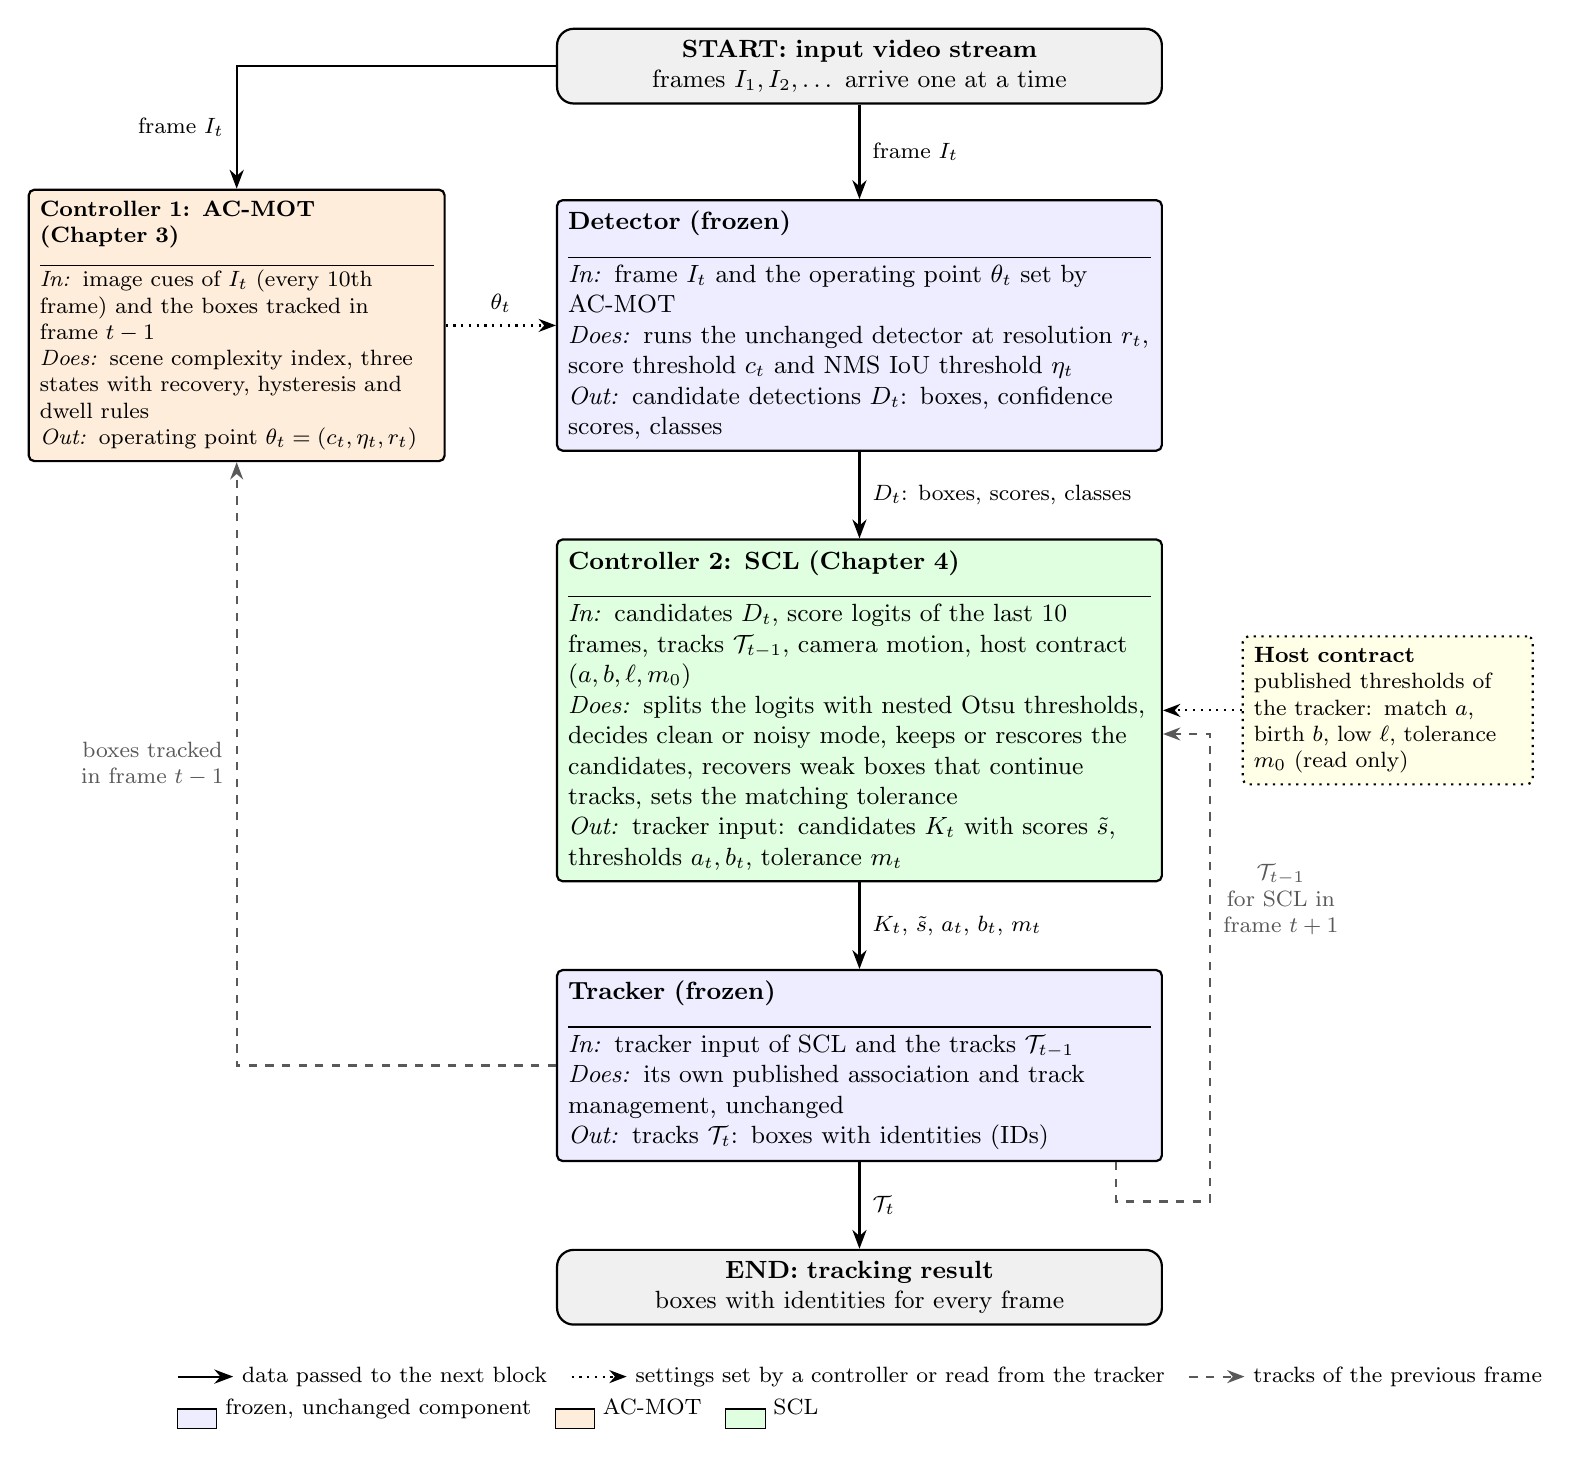
\begin{tikzpicture}[
  font=\small,
  io/.style={draw, thick, rounded corners=6pt, fill=gray!12, align=center, text width=74mm, inner sep=4pt},
  host/.style={draw, thick, rounded corners=2pt, fill=blue!7, align=left, text width=74mm, inner sep=4pt},
  c1/.style={draw, thick, rounded corners=2pt, fill=orange!14, align=left, text width=50mm, inner sep=4pt,
             font=\footnotesize},
  c2/.style={draw, thick, rounded corners=2pt, fill=green!12, align=left, text width=74mm, inner sep=4pt},
  set/.style={draw, dotted, thick, rounded corners=2pt, fill=yellow!10, align=left, text width=34mm,
              font=\footnotesize, inner sep=4pt},
  arr/.style={-{Stealth[length=2.4mm]}, thick},
  ctl/.style={-{Stealth[length=2.2mm]}, thick, dotted},
  fb/.style={-{Stealth[length=2.2mm]}, thick, dashed, black!65},
  lab/.style={font=\footnotesize, fill=white, inner sep=1.5pt, align=center}]
% main path, top to bottom
\node[io] (in) {\textbf{START: input video stream}\\ frames $I_1, I_2, \dots$ arrive one at a time};
\node[host, below=12mm of in] (det) {\blk{Detector (frozen)}
  {frame $I_t$ and the operating point $\theta_t$ set by AC-MOT}
  {runs the unchanged detector at resolution $r_t$, score threshold $c_t$ and NMS IoU threshold $\eta_t$}
  {candidate detections $D_t$: boxes, confidence scores, classes}};
\node[c2, below=11mm of det] (scl) {\blk{Controller 2: SCL (Chapter~4)}
  {candidates $D_t$, score logits of the last 10 frames, tracks $\mathcal{T}_{t-1}$, camera motion,
   host contract $(a,b,\ell,m_0)$}
  {splits the logits with nested Otsu thresholds, decides clean or noisy mode, keeps or rescores the
   candidates, recovers weak boxes that continue tracks, sets the matching tolerance}
  {tracker input: candidates $K_t$ with scores $\tilde{s}$, thresholds $a_t, b_t$, tolerance $m_t$}};
\node[host, below=11mm of scl] (trk) {\blk{Tracker (frozen)}
  {tracker input of SCL and the tracks $\mathcal{T}_{t-1}$}
  {its own published association and track management, unchanged}
  {tracks $\mathcal{T}_t$: boxes with identities (IDs)}};
\node[io, below=11mm of trk] (out) {\textbf{END: tracking result}\\ boxes with identities for every frame};
% controller 1 on the left of the detector
\node[c1, left=14mm of det] (ac) {\blk{Controller 1: AC-MOT\\(Chapter~3)}
  {image cues of $I_t$ (every 10th frame) and the boxes tracked in frame $t-1$}
  {scene complexity index, three states with recovery, hysteresis and dwell rules}
  {operating point $\theta_t=(c_t,\eta_t,r_t)$}};
% host contract on the right of SCL
\node[set, right=10mm of scl] (hc) {\textbf{Host contract}\\ published thresholds of the tracker:
  match $a$, birth $b$, low $\ell$, tolerance $m_0$ (read only)};
% arrows: data path
\draw[arr] (in) -- node[lab, right=1mm] {frame $I_t$} (det);
\draw[arr] (det) -- node[lab, right=1mm] {$D_t$: boxes, scores, classes} (scl);
\draw[arr] (scl) -- node[lab, right=1mm] {$K_t$, $\tilde{s}$, $a_t$, $b_t$, $m_t$} (trk);
\draw[arr] (trk) -- node[lab, right=1mm] {$\mathcal{T}_t$} (out);
\draw[arr] (in.west) -| node[lab, pos=0.75, left=1mm] {frame $I_t$} (ac.north);
% control and settings
\draw[ctl] (ac.east) -- node[lab, above=1mm] {$\theta_t$} (det.west |- ac.east);
\draw[ctl] (hc.west) -- (scl.east |- hc.west);
% feedback: tracks of the previous frame
\draw[fb] (trk.west) -| node[lab, pos=0.75, left=1mm] {boxes tracked\\in frame $t-1$} (ac.south);
\draw[fb] ($(trk.south east)+(-6mm,0)$) -- ++(0,-5mm) -| ([xshift=6mm]trk.east)
  |- node[lab, pos=0.25, right=1mm] {$\mathcal{T}_{t-1}$\\for SCL in\\frame $t+1$}
  ([yshift=-3mm]scl.east);
% legend
\node[font=\footnotesize, align=left, anchor=north] at ($(out.south)+(0,-4mm)$) {%
  \tikz[baseline=-0.6ex]\draw[arr] (0,0) -- (7mm,0); data passed to the next block\quad
  \tikz[baseline=-0.6ex]\draw[ctl] (0,0) -- (7mm,0); settings set by a controller or read from the tracker\quad
  \tikz[baseline=-0.6ex]\draw[fb] (0,0) -- (7mm,0); tracks of the previous frame\\[2pt]
  \tikz[baseline=-0.6ex]\node[draw, fill=blue!7, minimum width=5mm, minimum height=2.5mm] {}; frozen, unchanged component\quad
  \tikz[baseline=-0.6ex]\node[draw, fill=orange!14, minimum width=5mm, minimum height=2.5mm] {}; AC-MOT\quad
  \tikz[baseline=-0.6ex]\node[draw, fill=green!12, minimum width=5mm, minimum height=2.5mm] {}; SCL};
\end{tikzpicture}
\end{document}
